\documentclass{article}
\usepackage[margin = 2.54cm]{geometry} % set margin to traditional doc

%packages
\usepackage{graphicx} % Required for inserting images
\usepackage[most]{tcolorbox} %for creating environments
\usepackage{amsmath}
\usepackage{amssymb}
\usepackage{mathtools}
\usepackage{verbatim}
\usepackage[utf8]{inputenc}
\usepackage[dvipsnames]{xcolor} %for importing multiple colors
\usepackage{hyperref} %for creating links to different sections

\linespread{1.2} %controlling line spread

%define colors i like
\definecolor{myTeal}{RGB}{0,128,128}
\definecolor{myGreen}{RGB}{34,170,34}
\definecolor{mySapphire}{RGB}{15,82,186}
\definecolor{myEmerald}{RGB}{50.4, 130, 90}

%create math environments, can add [section] or [subsection] to add index counter based on sections/subsections
\newtheorem{define}{Definition}
\newtheorem{prop}{Proposition}
\newtheorem{thm}{Theorem}
\newtheorem{question}{Question}
\newtheorem{lemma}{Lemma}
\newtheorem{derive}{Derivation}

%setup colored box environment for each math env above
\tcolorboxenvironment{define}{
    enhanced, colframe=myTeal!50!teal, colback=myTeal!10,
    arc=5mm, lower separated=false, fonttitle=\bfseries, breakable
}
\tcolorboxenvironment{prop}{
    enhanced, colframe=myGreen!50!black, colback=myGreen!15,
    arc=5mm, lower separated=false, fonttitle=\bfseries, breakable
}
\tcolorboxenvironment{thm}{
    enhanced, colframe=mySapphire!50!mySapphire, colback=mySapphire!15,
    arc=5mm, lower separated=false, fonttitle=\bfseries, breakable
}
\tcolorboxenvironment{question}{
    enhanced, colframe=blue!50!black, colback=blue!10,
    arc=5mm, lower separated=false, fonttitle=\bfseries, breakable
}
\tcolorboxenvironment{lemma}{
    enhanced, colframe=myEmerald!50!myEmerald, colback=myEmerald!10,
    arc=5mm, lower separated=false, fonttitle=\bfseries, breakable
}
\tcolorboxenvironment{derive}{
    enhanced, colframe=myEmerald!50!myEmerald, colback=myEmerald!10,
    arc=5mm, lower separated=false, fonttitle=\bfseries, breakable
}

%setup hyperlink within pdf
\hypersetup{
    colorlinks=true,
    linkcolor=blue,
    filecolor=magenta,      
    urlcolor=cyan,
    pdftitle={Overleaf Example},
    pdfpagemode=FullScreen,
}

%common command (add to template)
%general
\newcommand{\FF}{\mathbb{F}}
\newcommand{\NN}{\mathbb{N}}
\newcommand{\ZZ}{\mathbb{Z}}
\newcommand{\QQ}{\mathbb{Q}}
\newcommand{\RR}{\mathbb{R}}
\newcommand{\CC}{\mathbb{C}}

\newcommand{\Id}{\textmd{Id}} %identity
\newcommand{\lcm}{\textmd{lcm}}
\DeclarePairedDelimiter{\abs}{\lvert}{\rvert}
\DeclarePairedDelimiter{\norm}{\lVert}{\rVert}
\DeclarePairedDelimiter{\paran}{(}{)}%paranthesis
\DeclarePairedDelimiter{\bracket}{\langle}{\rangle}

%algebra
\newcommand{\Gal}{\textmd{Gal}}
\newcommand{\Aut}{\textmd{Aut}}
\newcommand{\End}{\textmd{End}}
\newcommand{\Coker}{\textmd{Coker}}
\newcommand{\Hom}{\textmd{Hom}}
\newcommand{\Nil}{\textmd{Nil}}
\newcommand{\Char}{\textmd{char}}

%analysis
\newcommand{\Vol}{\textmd{Vol}}

%complex
\newcommand{\Real}{\textmd{Re}}
\newcommand{\Imag}{\textmd{Im}} %can also be used for Image
\newcommand{\Res}{\textmd{Res}}

%lie algebra
\newcommand{\gl}{\mathfrak{gl}}

%physics
\newcommand{\br}{\textbf{r}} %position
\newcommand{\bv}{\textbf{v}} %velocity
\newcommand{\ba}{\textbf{a}} %cceleration
\newcommand{\bF}{\textbf{F}} %force
\newcommand{\bP}{\textbf{P}} %momentum
\newcommand{\bL}{\textbf{L}} %angular momentum
\newcommand{\bN}{\textbf{N}} %torque
\newcommand{\bw}{\textbf{w}} %angular velocity
\newcommand{\bzero}{\textbf{0}}

%four-vectors for relativity
\newcommand{\bA}{\textbf{A}}
\newcommand{\bB}{\textbf{B}}
\newcommand{\bC}{\textbf{C}}
\newcommand{\bD}{\textbf{D}}


\title{Phys 103 HW4}
\author{Zih-Yu Hsieh}

\begin{document}
\maketitle

\section*{1}
\begin{question}\label{q1}
    An algebraic expression is said to be \emph{Lorentz covariant} if its form is the same in all inertial frame: the expression differs in two inertial frames $F$ and $F'$ only by putting prime marks on all the coordinate labels. For example, $C_\mu = \eta_{\mu\nu}B^\nu$ and $D=A^\mu \eta_{\mu\nu}B^{\nu}$ are both Lorentz covariant, as you could show using 
    $$\hat{\Lambda}^T\hat{\eta}\hat{\Lambda}=\hat{\eta}$$
    Lorentz scalars (which are unchanged), Lorentz vectors ($V^{\mu'} = \Lambda^{\mu'}_{\ \ \mu}V^\mu$), and Lorentzz tensors (as many factors of the transformation as appropriate) are thus all examples of Lorentz covariant quantities. (For all of these, the prefix may be \emph{four-} instead of Lorentz, or it may be dropped entirely if not trying to emphasize the four dimensions). If $K$ is a four-scalar and $\textbf{A},\textbf{B},\textbf{C},\textbf{D}$ are all four-vectors, identify each of the following expressions as a scalar, vector, tensor, or non-covariant (and prove/explain):
    \begin{itemize}
        \item $F=KA^\mu B^\mu$
        \item $F=K \eta_{\mu\nu}A^\mu B^\nu$
        \item $F^{\mu\nu} = KA^\mu B^\nu$
        \item $F^\lambda = C^\lambda A^\mu \eta_{\mu\nu}B^\nu$
        \item $F^\lambda = C^\mu A^\lambda \eta_{\mu\nu}B^\nu$
        \item $F=KA^\mu \eta_{\mu\nu}B^\lambda \eta_{\lambda\sigma}C^\nu D^\sigma$
    \end{itemize}
\end{question}

\textbf{Pf:}
\begin{itemize}
    \item[1)] For the expression $F=KA^\mu B^\mu$, it in general is non-covariant: If expressed in matrix multiplication, the term $A^\mu B^\mu$ is a dot product of the Lorentz vectors $\textbf{A},\textbf{B}$, which in matrix form is as follow:
    \begin{align}
        F = K\textbf{A}^T\textbf{B}
    \end{align}
    Now, if change an inertial frame (the primed index) that has some relative speed with the original inertial frame (the unprimed index), then with $K$ being identical (since it's a Lorentz scalar / four-scalar), we get:
    \begin{align}
        F' = KA^{\mu'}B^{\mu'} = K(\hat{\Lambda}\textbf{A})^T (\hat{\Lambda}\textbf{B}) = K\textbf{A}^T(\hat{\Lambda}^T\hat{\Lambda})\textbf{B}
    \end{align}
    In general, $\hat{\Lambda}^T\hat{\Lambda}\neq \Id$ (identity matrix). Hence, in general $\textbf{A}^(\hat{\Lambda}^T\hat{\Lambda})\textbf{B}\neq \textbf{A}^T\textbf{B}$ in terms of matrix multiplication. For instance, take $\textbf{A}=(1,0,0,0)$, $\textbf{B}=(1,1,0,0)$ (in unprimed coordinates $(ct,x,y,z)$), we get:
    \begin{align}
        &F = K\bA^T\bB = K\\
        &F' = K\textbf{A}^T(\hat{\Lambda}^T\hat{\Lambda})\textbf{B} = K\textbf{A}^T\hat{\Lambda}^T\begin{pmatrix}
            \gamma - \gamma\beta \\ \gamma - \gamma\beta \\ 0 \\ 0
        \end{pmatrix} = (\gamma-\gamma\beta)K\textbf{A}^T\hat{\Lambda}\textbf{B} = (\gamma-\gamma\beta)^2K\textbf{A}^T\textbf{B} = (\gamma(1-\beta))^2K
    \end{align}
    (Note: (4) is entirely in Matrix notation, which $\bB$ is an eigenvector of $\hat{\Lambda}$ with eigenvalue $\gamma(1-\beta)$, and $\hat{\Lambda}^T=\hat{\Lambda}$).

    In general $(\gamma(1-\beta))^2\neq 1$ (since $(1-\beta)^2 \neq \paran{1-\beta^2}=\frac{1}{\gamma^2}$, the equality happens only at $\beta=0, \beta=1$, but $\beta=1$ implies $\frac{v}{c}=1$, which is not valid to say in special relativity), so for the above $F\neq F'$.

    \rule{15.6cm}{0,1mm}

    \item[2)] For $F=K \eta_{\mu\nu}A^\mu B^\nu = KA^\mu \eta_{\mu\nu}B^\nu$, it's a Lorentz Scalar: In matrix form it can be written as $F=K\textbf{A}^T\hat{\eta}\textbf{B}$. Which, under some arbitrary inertial frame (primed index) which is transformed from the original frame (unprimed index) using transformation $\hat{\Lambda}$, with $K$ being fixed, we get:
    \begin{align}
        F' = KA^{\mu'}\eta_{\mu'\nu'}B^{\nu'} = K(\hat{\Lambda}\textbf{A})^T\hat{\eta}(\hat{\Lambda}\textbf{B}) = K\textbf{A}^T(\hat{\Lambda}^T\hat{\eta}\hat{\Lambda})\textbf{B} = K\textbf{A}^T\hat{\eta}\textbf{B} = F
    \end{align}
    (Note: Recall that $\hat{\Lambda}^T\hat{\eta}\hat{\Lambda}=\hat{\eta}$).

    So, under arbitrary Lorentz transformation, such term is fixed as a scalar, which is a Lorentz scalar.

    \rule{15.6cm}{0,1mm}

    \item[3)] For $F^{\mu\nu}=KA^\mu B^\nu$, it's a Lorentz tensor: If consider $\hat{F}$ as the matrix representation of $F^{\mu\nu}$, then we get the following form:
    \begin{align}
        \hat{F} = K\bA \bB^T
    \end{align}
    Which, under the primed frame, we get:
    \begin{align}
        F^{\mu'\nu'} = KA^{\,u
        }B^{\nu'},\quad \textmd{In matrix form: } K(\hat{\Lambda}\bA)(\hat{\Lambda}\bB)^T = \hat{\Lambda}(K\bA \bB^T)\hat{\Lambda}^T = \hat{\Lambda}\hat{F}\hat{\Lambda}^T
    \end{align}
    Which, if consider two transformations, $F^{\mu\nu}$ turns out to follow certain transformations, can be determined as a tensor.
    (Can be determined using an isomorphism to $K\bA \otimes \bB$, where the transformation is $\hat{\Lambda}\otimes \hat{\Lambda}$).

    \rule{15.6cm}{0,1mm}

    \item[4)] For $F^\lambda = C^\lambda A^\mu \eta_{\mu\nu}B^\nu$, it is a Lorentz vector: Recall that $K =  A^\mu \eta_{\mu\nu}B^\nu$ is proven to be a Lorentz scalar in 2), hence for $F^\lambda = K C^\lambda$, let $\bF$ be the four-dimensional vector representation of coordinates $F^\lambda$, then we get that $\bF = K\bC$ (where $\bF$ is the Lorentz vector $\bC$ scaled with a factor of Loretz scalar $K$), which satisfies the following:
    \begin{align}
        \hat{\Lambda}\bF = \hat{\Lambda}(K\bC) = K(\hat{\Lambda}\bC)
    \end{align}
    Since the right side expression has index notation of $K(\Lambda^{\mu'}_{\ \mu} C^\mu) = KC^{\mu'} = F^{\mu'}$ (based on the definition of Lorentz vector and $F^\mu$), then we can see that $F^{\mu'}$ can be obtained through Lorentz Transformation of $F^\mu$, hence it's a Lorentz vector.

    \rule{15.6cm}{0,1mm}

    \item[5)] For $F^\lambda = C^\mu A^\lambda \eta_{\mu\nu}B^\nu = A^\lambda(C^\mu\eta_{\mu\nu}B^\nu)$, notice that swap $\textbf{A}$ and $\textbf{C}$, it is identical to 4) (right above), so it is also a Lorentz vector.
    
    \rule{15.6cm}{0,1mm}

    \item[6)] For $F=KA^\mu \eta_{\mu\nu}B^\lambda \eta_{\lambda\sigma}C^\nu D^\sigma = K(A^\mu\eta_{\mu\nu}C^\nu)(B^\lambda\mu_{\lambda\sigma}D^\sigma)$, since in the problem with any four vectors $\textbf{U},\textbf{V}$, the term $U^\mu\eta_{\mu\nu}V^\nu$ is a Lorentz scalar (also proven in 2)), then $F$ is in fact a product of three Lorentz scalars. In any frame, these three scalars are fixed, so $F$ is also fixed, showing that it's also a Lorentz scalar.
\end{itemize}

\break

\section*{2}
\begin{question}\label{q2}
    Al and Bert are identical twins. When Bert is 24 years old, he travels to a distant planet at speed $\frac{12}{13}c$, turns around, and heads back at the same peed, arriving home at age $44$. Al stays at home. How old is Al when Bert returns? How far away was the planet in Al's frame? Why can't Bert reasonably claim that from his point of view it was Al who was moving, so that Al's clocks should be dilated, making Al younger than Bert when they reunite? (Make sure to give a reasonably thorough ansewr; rather than just a quick statement, you should consider what's going on in some different frames and why certain calculations or interpretations fail).
\end{question}

\textbf{Pf:}

For this problem, we can make a few premises: First, assume Bert is traveling in $x$-direction in Al's frame (unprimed), while during the forward trip Bert's frame is denoted using $x'$ (primed), while the backward trip Bert's frame is denoted using $x''$ (double primed). And, for simplicity, we'll use year for time scale.

\hfil

First, since Bert travels to a planet and comes back, in Al's frame Bert travels through two identical distance; and, since for both trips, Bert's relative speed to Al is $\frac{12}{13}c$ (in different direction), both trips (except the part of changing direction) are identical. Hence can assume for both trips in Bert's frame, he travels the same distance, while both trips take the same time in Bert's frame. Then, since for the two trips, in Bert's frame he changes from 24 to 44 years old, so in Bert's frame he passes through total of 20 years, with the two trips being similar (only different in direction), each trip takes $\Delta t'=\Delta t'' = 10$ years in Bert's frame. 

\begin{comment}
Bert observes the planet heading towards him with speed $\frac{12}{13}c$, hence in Bert's frame, the planet travels through distance $\Delta x' = \frac{12}{13}c \cdot 10$, where it's with unit m/s times year.


Here, with speed $\frac{12}{13}c$, we get $\beta = \frac{12}{13}c/c = \frac{12}{13}$, and $\gamma = \frac{1}{\sqrt{1-\beta^2}} = \frac{13}{5}$. Since it is the distance that is traveling in Bert's frame, if the original distance (between Al and the planet) is $\Delta x$, by length contraction $\Delta x' = \frac{\Delta x}{\gamma}$, or $\Delta x=\gamma\Delta x' = \frac{13}{5}\frac{120}{13}c = 24c$ m/s times year.
\end{comment}

Using the first trip as example, in Bert's frame, the event of him reaching the planet has coordinates $(ct', x') = (c\Delta t', \Delta x') = (10c, 0)$ (both are with unit of m/s times year; since in Bert's frame he never moves, so $x'=0$, and because Bert starts at $(ct',x')=(0,0)$ in his own frame, then the eventual $ct'= c\Delta t'$). Hence, if this event of Bert reaching the planet has coordinate $(ct, x)$ in Al's frame, using Lorentz boost, we get:
\begin{align}
    \begin{pmatrix}
        10c\\
        0
    \end{pmatrix} = \begin{pmatrix}
        ct'\\x'
    \end{pmatrix} = \begin{pmatrix}
        \gamma & -\gamma\beta\\
        -\gamma\beta & \gamma
    \end{pmatrix}\begin{pmatrix}
        ct\\x
    \end{pmatrix} = \begin{pmatrix}
        \frac{13}{5}\paran*{ct - \frac{12}{13}x}\\
        \frac{13}{5}\paran*{x - \frac{12}{13}ct}
    \end{pmatrix} = \begin{pmatrix}
        \frac{13}{5}ct - \frac{12}{5}x\\
        \frac{13}{5}x - \frac{12}{5}ct
    \end{pmatrix}
\end{align}
(Note: above both have units of m/s times year).

Which, solving the system of equations, we get (both in units of m/s times year):
\begin{align}
    x= 24c,\quad ct = \frac{313}{13}c
\end{align}
Which, this is the coordinate of Bert reaching the planet in Al's frame, which the $x$ coordinate is the planet's distance from Al. Transfer the distance to light year, in Al's frame the planet has coordinate $x=24$ light years.

Hence, with Bert's speed being $\frac{12}{13}c$ m/s, in Al's frame, it takes Bert $\Delta t = \frac{\Delta x}{v} = \frac{24c}{\frac{12}{13}c} = 26$ years to reach the planet. And, since for Bert's trip back it's a similar system (after changing coordinates), it takes a total of $2\cdot 26 = 52$ year for Bert to travel back and forth in Al's frame. At this point, in Al's frame himself is $24 + 52 = 76$ years old.

\rule{15.6cm}{0.1mm}

The reason why Bert can't claim that Al's clock is the one dilated (which supposedly should cause Al to be younger than Bert when reunite), is because Bert is not in an inertial frame: Even though we assumed the change of direction to happen in an instant, but realistically during that moment Bert is in fact accelerating with respect to Al and the Planet, which makes him no longer in an inertial frame, and cause the calculation to be more complicated.

If we consider Bert's frame \textbf{only} in the first trip, about what the second trip looks like, we'll get the following: 

We know for the second trip (in its own frame, with double prime coordinates) has the difference in coordinates (of the end and the start) given as $(c\Delta t'', \Delta x'') =   (10c, 0)$ (in the second trip's frame, Bert isn't moving, so $\Delta x'' = 0$, while time passes through $\Delta t''=10$ years). Then, because the second trip Bert has relative speed of $\frac{12}{13}c$ in $-x$ direction of Al's frame, we get the following relation about the difference of coordinates in Al's frame:
\begin{align}
    \begin{pmatrix}
        c\Delta t''\\ \Delta x''
    \end{pmatrix}=\begin{pmatrix}
        \gamma & \gamma\beta\\
        \gamma\beta & \gamma
    \end{pmatrix}\begin{pmatrix}
        c\Delta t\\ \Delta x
    \end{pmatrix}\implies 
    \begin{pmatrix}
        c\Delta t\\\Delta x
    \end{pmatrix} = \begin{pmatrix}
        \gamma & -\gamma\beta\\
        -\gamma\beta & \gamma
    \end{pmatrix}\begin{pmatrix}
        c\Delta t''\\\Delta x''
    \end{pmatrix}
\end{align}
Then again, since during the first trip (the primed frame) has relative speed of $\frac{12}{13}c$ in $x$ direction based on Al's frame, we get:
\begin{align}
    \begin{pmatrix}
        c\Delta t'\\\Delta x'
    \end{pmatrix} = \begin{pmatrix}
        \gamma & -\gamma\beta\\
        -\gamma\beta & \gamma
    \end{pmatrix}\begin{pmatrix}
        c\Delta t\\\Delta x
    \end{pmatrix} = \begin{pmatrix}
        \gamma & -\gamma\beta\\
        -\gamma\beta & \gamma
    \end{pmatrix}^2 \begin{pmatrix}
        c\Delta t''\\\Delta x''
    \end{pmatrix} = \begin{pmatrix}
        \gamma^2(1+\beta^2) & -2\gamma^2\beta\\
        -2\gamma^2\beta & \gamma^2(1+\beta^2)
    \end{pmatrix}\begin{pmatrix}
        c\Delta t''\\\Delta x''
    \end{pmatrix}
\end{align}
With $\gamma = \frac{13}{5}$, $\beta = \frac{12}{13}$, $\Delta x''=0$, and $\Delta t''=10c$, we get the following for $\Delta t'$ (in m/s times years):
\begin{align}
    &c\Delta t' = \gamma^2(1+\beta^2)c\Delta t'' - 2\gamma^2\beta \Delta x'' = \frac{13^2}{5^2}\paran*{1+\frac{12^2}{13^2}}10c = \frac{3130}{25}c\\
    &\implies \Delta t' = \frac{3130}{25}\textmd{ years} = 125.2 \textmd{ years}
\end{align}
Which, adding the first trip's $10$ years, in the first trip's frame, Bert takes total of $135.2$ years to travel, which is significantly longer than the time that Al perceived to pass (which is 52 years). 

\begin{comment}
Moreover, if using time dilation formula, since Al is the one moving in speed $\frac{12}{13}c$ (with $\gamma = \frac{13}{5}$), then with $\Delta t=52$ years as Al's percieved time difference, Bert (in the first trip's frame) would percieve a time of $\Delta t' = \gamma \Delta t = \frac{13}{5}\cdot 52 = 135.2$ years, which matches with the calculated time in the first trip's frame.
\end{comment}

Hence, time dilation in fact is applied (when Bert sticked with an inertial fram, in this calculation the first trip's frame), the reason why we can't see it in Bert's perspective, is because the additional time of the trip can only be seen in the second trip \textbf{if Bert stays in the first trip's frame}. However, since Bert changes his direction of travel, he no longer stays in the same frame, hence the time dilation effect can no longer be seen. (This also tells us that time dilation can only be applied when objects are staying in inertial frame; if change of direction happens, it no longer applies).

\break

\section*{3}
\begin{question}\label{q3}
    Cookie dough lies on a conveyer belt that moves at speed $v$. A circular stamp of radius $r$ stamps out cookies as the dough rushes by beneath it. When you buy these cookies in a store, what shape are they? If you think they're not circular, be sure to say (and explain) whether they're squashed or stretched relative to the samp. Explain what's going on from both cookie's and the stamp's perspective.
\end{question}

\textbf{Pf:}

For this question, assume the cookie dough never deforms (i.e. in either frame of the stamp or the cookies, the cookies never change its size). 

Also, it's important to verify which frame it is when the stamp cuts the cookies: Here, we'll assume that the stamp lands on the cookie dough "simultaneously" in the stamp's frame (i.e. the whole stamp lands on the cookie dought at the same time $t_0$ in the stamp's frame).

We'll assume that the cookie dough is traveling in $x$ direction of the stamp's frame.

\subsection*{1) In the Stamp's Frame:}
Since we assume that the stamp's area touches the dough simultaneously in the stamp's frame, then the important part is the dough's length (in traveling direction) in the stamp's frame. 

If assume both frames are inertial (or the relative speed never changes), then with $\Delta t=0$ (for stamping process) in the stamp's frame, length contraction can be applied. Because the dough is moving relative to the stamp, then the length of the dough has contracted in the stamp's frame (while the width in the orthogonal direction doesn't). So, the stamp would cover a larger portion of the length of the dough, while the width wasn't affected. 

Then, when the cookies are bought in a store, the length of the stamp would be longer, showing a shape of an elllipse (or, the circular stamp is stretched in the moving direction on the dough). More precisely, with the length of the stamp being $2r$ in the stamp's frame (when being cut), suppose this length is $x$ when the cookie is at rest, then based on length contraction, with its distance (when the dough is moving) being $2r$, we get $2r = \frac{x}{\gamma}$, so $x = \gamma 2r = \frac{2r}{\sqrt{1-\frac{v^2}{c^2}}}$.

\begin{figure}[h!]
    \begin{center}
        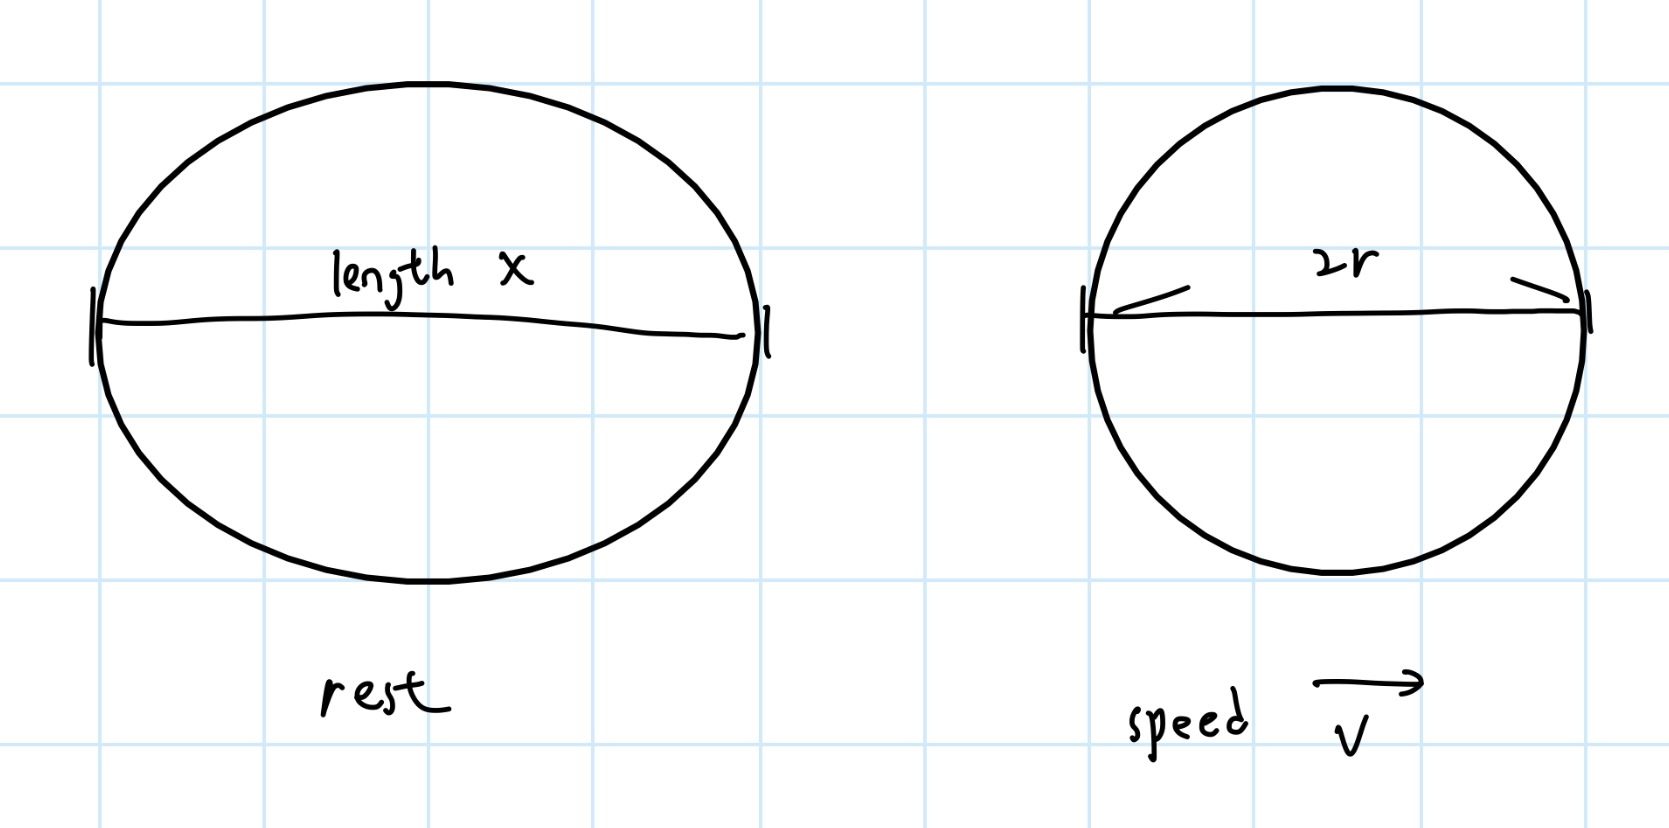
\includegraphics[width=90mm]{hw4 q31.jpg}
        \caption{Illustration of the cookie under different frames}
    \end{center}
\end{figure}

\subsection*{2) In the Cookie Dough's Frame:}
Intuitively, if we think about the cookie dough's frame, because the stamp is the one moving, then applying length contraction, the stamp should have a length shorter than usual, so if "simultaneously" stamp the stamp on the cookie dough (in the dough's frame), it should be an ellipse with the length shrinked.

But, the problem is, if we assume we're stamping on the dough "simultaneously" in the stamp's frame, this set of events (where the points on the stamp touches the points on the dough) appears to not be "simultaneous" in the cookie dough's frame, which can be seen from the following spacetime diagram:

\begin{figure}[h!]
    \begin{center}
        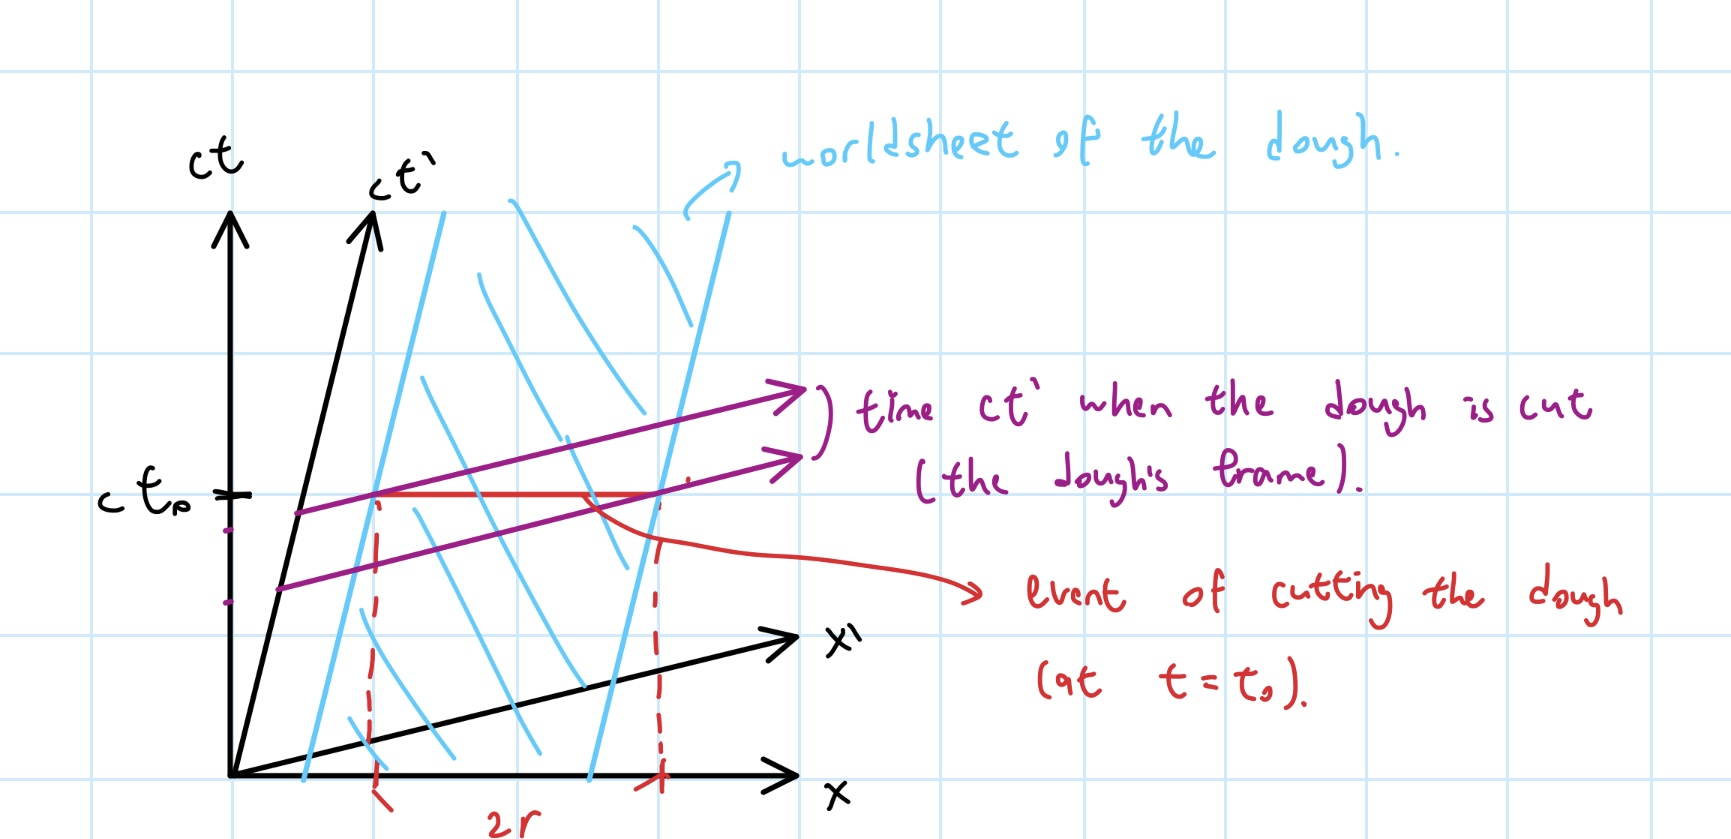
\includegraphics[width=100mm]{hw4 q32.jpg}
        \caption{Spacetime Diagram of the cutting events}
    \end{center}
\end{figure}

Because the stamping process doesn't appear to be "simultaneous" in the cookie dough's frame, since from the Spacetime diagram we can see that different parts of the stamp touches the dough at different time, so even though the "length" of the stamp is shorter in the dough's frame, it also needs to take into account that between small "instant" in the dough's frame, the stamp also travels, hence the total length of the dough after cutting needs to take into account of the distance the stamp has traveled. Then, we can't directly apply length contraction here, which causes no contradiction from the previous part.

\hfil

Overall, we can say that the cookie appears to be an ellipse, which is stretched in the cookie dough's traveling direction (if we assume the stamping process is "simultaneous" in the stamp's frame), with length $\frac{2r}{\sqrt{1-\frac{v^2}{c^2}}}$ (while the width is still $2r$).

\break

\section*{4}
\begin{question}\label{q4}
    A stick of proper length $L$ moves at speed $v$ in the direction of its length. It passes over an infinitesimally thin sheet that has a hole of diameter $L$ cut in it. As the stick passes over the hole, the sheet is raised so that the stick passes through the hole and ends up underneath the sheet. Well, maybe\dots

    In the lab frame, the stick's length is contracted to$L/\gamma$, so it appears to easily make it through the hole. But in the stick frame, the \emph{hole} is contracted to $L/\gamma$, so it appears that the stick does \emph{not} make it through the hole (or rather, the hole doesn't make it around the stick, since the hole is what is moving in the stick frame). So the question is: does the stick end up on the other side of the sheet or not?

    Once you have that question figured out, also consider this variant: suppose it's not a sheet, but a table (still with a hole of proper length $L$). The stick slides along the table at speed $v$; does it make it across the gap?
\end{question}

\textbf{Pf:}

\subsection*{Thin Sheet Problem:}
Here, it is more important to understand the simultaneity when the stick passes through the hole (like in Question \ref{q3}, the simultaneity of the stamping process). Based on the description, since when the stick passes over the hole, the sheet is raised for the stick to pass through the hole, can assume it's intended for every part of the stick simultaneously passes through the hole in the lab frame.

So, using the lab frame, with the stick's length contracted to $L/\gamma<L$, the stick would have no problem passing through the hole.

\hfil

If we turn to the stick's frame, intuitively using length contraction, we'd get that the hole contracts to length $L/\gamma<L$, so it's not possible for the stick to pass through the hole "simultaneously" in the stick's frame; however, because the simultaneity in the lab frame records a different set of events (or different set of the parts of the sticks) in spacetime, being simultaneous in the lab frame is different from being simultaenous in the stick's frame. So, the stick is not passing through the hole "simultaneously" in the stick's frame. This can also be seen in the following spacetime diagram:

\begin{figure}[h!]
    \begin{center}
        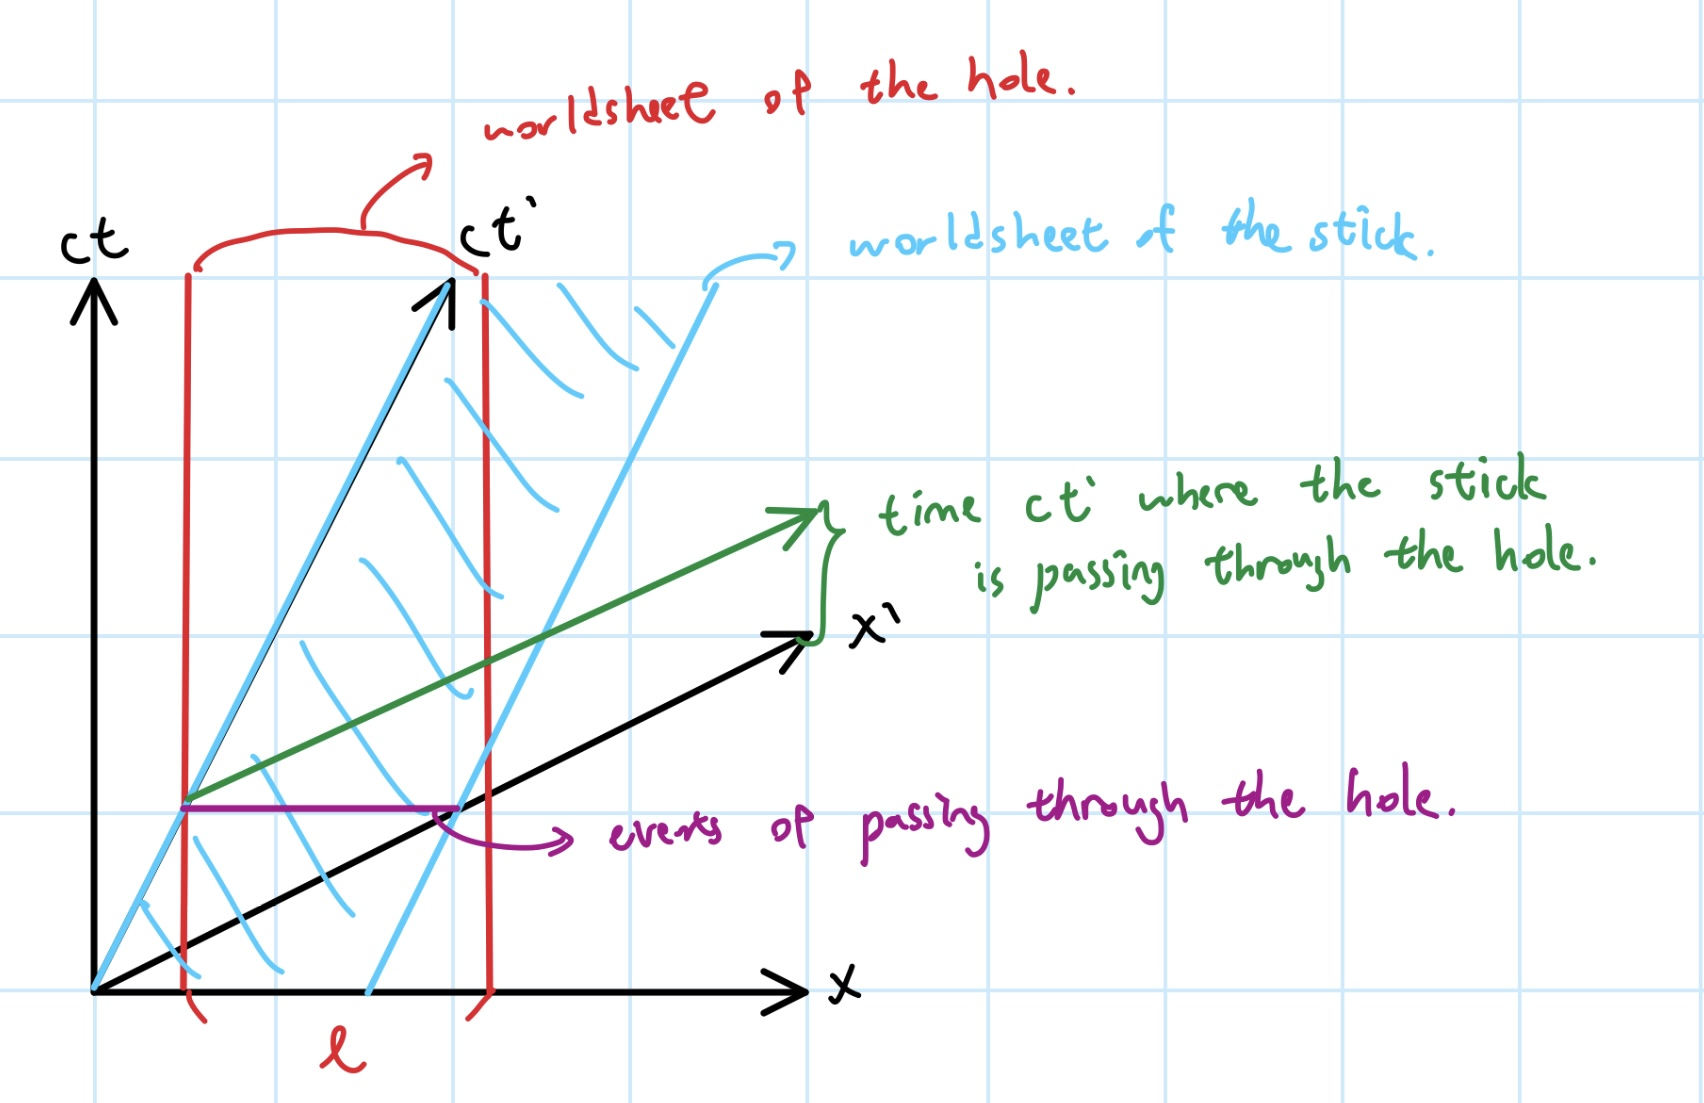
\includegraphics[width=78mm]{hw4 q41.jpg}
        \caption{Spacetime Diagram of the events}
    \end{center}
\end{figure}

So, one can see in the Spacetime Diagram, that in the stick's frame, it isn't passing through the hole at the same time, but gradually having more parts passing through the hole, showing that the stick can still pass through the hole in the stick's frame, just not passing through simultaneously.

\subsection*{Table Problem:}

\begin{figure}[h!]
    \begin{center}
        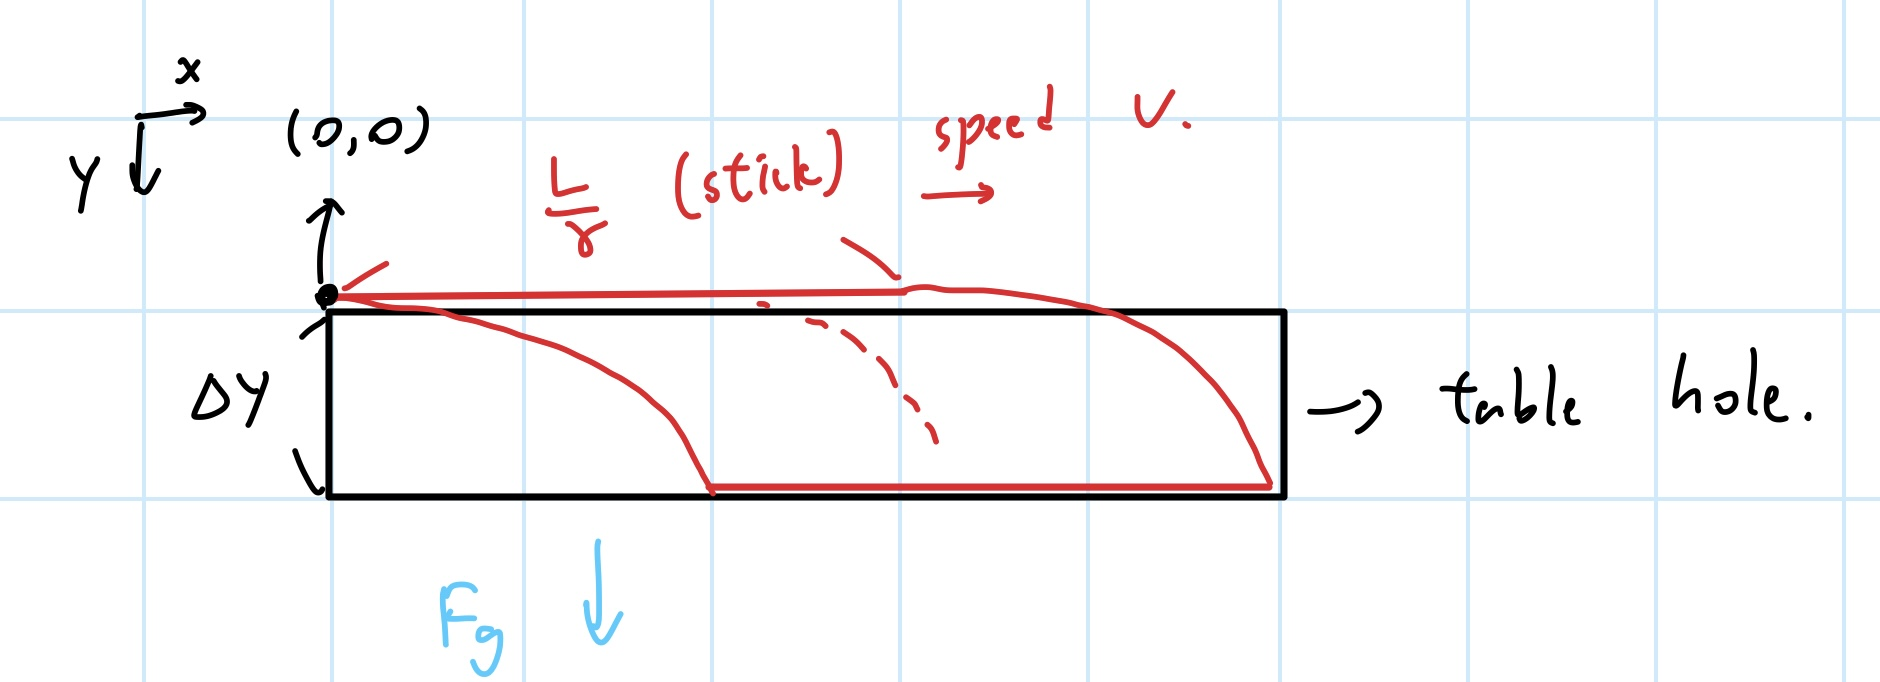
\includegraphics[width=100mm]{hw4 q42.jpg}
        \caption{The Illustration of how the stick passes through the hole}
    \end{center}
\end{figure}

If we consider the stick with proper length $L$, sliding on a table with a hole with proper length $L$ (and some thickness $\Delta y$ in the original frame), and the stick intends to fall through the hole when the whole body is simultaneously on top of the hole in the original frame (can make this assumption if the stick is fast enough, such that the center of mass loses the table's support approximately when the whole stick is above the hole).

Then, it'll create some velocity in the orthogonal direction due to gravity (in the original frame). However, notice that this new velocity has component that is orthogonal to the original traveling direction (where the length is placed), so it's not affecting the length, hence in the rest frame we still have the stick contracts to length $L/\gamma$ (i.e. length contraction only occurs in the traveling direction of the object). 

Which, back to the kinematics, suppose for the stick to fall through the thickness of the table $\Delta y$, since initially the vertical speed is $0$, with acceleration $g$, its vertical motion is recorded as $\frac{1}{2}gt^2$. So, if at time $t$ it falls through the distance $\Delta y$, we get $\frac{1}{2}gt^2=\Delta y$, or $t=\sqrt{\frac{2\Delta y}{g}}$. During this time, the stick travels horizontally of distance $vt = v\sqrt{\frac{2\Delta y}{g}}$, then the head of the stick is at position $L/\gamma + v\sqrt{\frac{2\Delta y}{g}}$. If we want the stick to pass through the hole, we want $L/\gamma + v\sqrt{\frac{2\Delta y}{g}}\leq L$, which $\sqrt{\frac{2\Delta y}{g}} \leq \frac{(\gamma -1)L}{\gamma v}$. This implies $\frac{2\Delta y}{g} \leq \frac{(\gamma-1)^2L^2}{\gamma^2 v^2}$, hence $\Delta y\leq \frac{g(\gamma-1)^2L^2}{2\gamma^2 v^2}$. 

This thickness is the limiting condition for the stick to actually pass through the hole.

\break

\section*{5}
\begin{question}\label{q5}
    Two spaceships float in space and are at rest relative to each other a distance $\ell$ apart. They are connected by a string of unstretched length $\ell$. The string can stretch somewhat, but it can't withstand an arbitrary amount of stretching. In the inertial frame which is initially the rest frame of the spaceships, at a given instant, the spaceships simultaneously begin accelerating in the same direction (along the line between them) with uniform acceleration. (In other words, assume they have identical engines and put them on the same setting). Consider the following two arguments:
    \begin{itemize}
        \item Take the entire contraption of the two ships and the string, considered to be one object. The proper length of this object is $\ell$. Therefore, when it's moving at some speed $v$, its length in the initial rest frame is contracted to $\ell/\gamma$. The string is thus always at its unstretched length, no matter how fast the ships are going, so it never breaks.
        \item Since they start at the same speed and have the same acceleration, the two ships are always moving at the same speed. Therefore, the distance between them (in the initial frame) is always $\ell$. When the string is moving at speed $v$, its length when unstretched in $\ell/\gamma$; it is therefore stretched by a factor $\gamma$ as long as it connects the two ships. After enough time, $\gamma$ will be large enough that the string breaks.
    \end{itemize}
    Which is correct? Or are both wrong? Make sure to support your answer with a thorough argument; in particular, you might consider what's going on in \emph{other} frames.
\end{question}

\textbf{Pf:}

First, we'll consider the worldline of the two spaceships: In the initial rest frame (denote as $F$), we can assume at $t=0$, spaceship 1 has $x$ coordinate $x_1(0)=0$, which spaceship 2 has $x$ coordinate $x_2(0)=\ell + x_1(0) = \ell$. Then, because both spaceships are at rest when $t=0$, and both has uniform acceleration $a$, then we get that $v_1(t)=v_2(t) = at$ in frame $F$ (which, with $v(t)<c$, showing that $t < \frac{c}{a}$). Then, we get that $x_1(t) = \frac{1}{2}at^2$ and $x_2(t) = \frac{1}{2}at^2 + \ell$ based on the initial conditions. Hence, with the $ct$ and $x$ coordinates, the set $\{(ct,\frac{1}{2}at^2)\ |\ 0\leq t<\frac{c}{a}\}$ is the worldline of the first spaceship, while $\{(ct,\frac{1}{2}at^2+\ell)\ |\ 0\leq t<\frac{c}{a}\}$ is the worldline of the second spaceship. This also shows that the distance between the two spaceships is $(\frac{1}{2}at^2+\ell)-\frac{1}{2}at^2=\ell$ at any time $0\leq t<\frac{c}{a}$ (in frame $F$). This proves that the first statement is wrong, since in the initial rest frame, the length is no $\frac{\ell}{\gamma}$, but maintains as $\ell$.

\hfil

Then, to consider the change in rope's length, we need to consider the frame of one of the spaceships (we'll use the first spaceship here): In frame $F$, for any time $t_0\geq 0$, the coordinates of spaceship $1$ is $(ct_0, \frac{1}{2}at_0^2)$ and with speed $v=at_0$ in $x$ direction (so $\beta = \frac{at_0}{c}$ at this event). Which, using Lorentz Boost, we get that the difference of events from spaceship 1 in each coordinate of spaceship 1's frame is as follow:
\begin{align}
    \begin{pmatrix}
        c\Delta t'\\\Delta x'
    \end{pmatrix} = \begin{pmatrix}
        \gamma & -\gamma\beta\\ -\gamma\beta&\gamma
    \end{pmatrix}\begin{pmatrix}
        c\Delta t\\\Delta x
    \end{pmatrix} = \begin{pmatrix}
        \gamma c\Delta t-\gamma\beta \Delta x\\ -\gamma\beta c\Delta t + \gamma\Delta x
    \end{pmatrix}
\end{align}
If we fix the time at $t=t_0$ in frame $F$, and measure the rope's two ends (one at spaceship 1, one at spaceship 2), then we get $\Delta t=0$, while $\Delta x=\ell$. Hence, in spaceship 1's frame, we get the two spaceships having distance $\Delta x' = -\gamma\beta c\Delta t+\gamma\Delta x = \gamma \ell$. So, the string is stretched from length $\ell$ to length $\gamma\ell$ in spaceship 1's frame. This indicates that the second statement describes a more accurate scenario of what's happening to the spaceships and the string.

\hfil

However, if we want a more accurate situation, notice that in the above case $c\Delta t' = \gamma c\Delta t-\gamma\beta \Delta x = -\gamma\beta\ell \neq 0$, hence showing that the measurement of the string's length is not made at the same instant in spaceship 1's frame. However, to make the measurement at the same instant, because of the accelerated nature, it's hard to calculate.

So, to simplify the situation, we'll create a new scenario: Assume at time $t_0$ in original frame $F$, the two spaceships suddenly stops accelerating. Then, their worldline would follow the tangent lines of the original worldline (since the velocity in frame $F$ is determined by the moment they stop accelerating). Then, the following is the worldlines of this new scenario (while also including the original worldlines):

\begin{figure}[h!]
    \begin{center}
        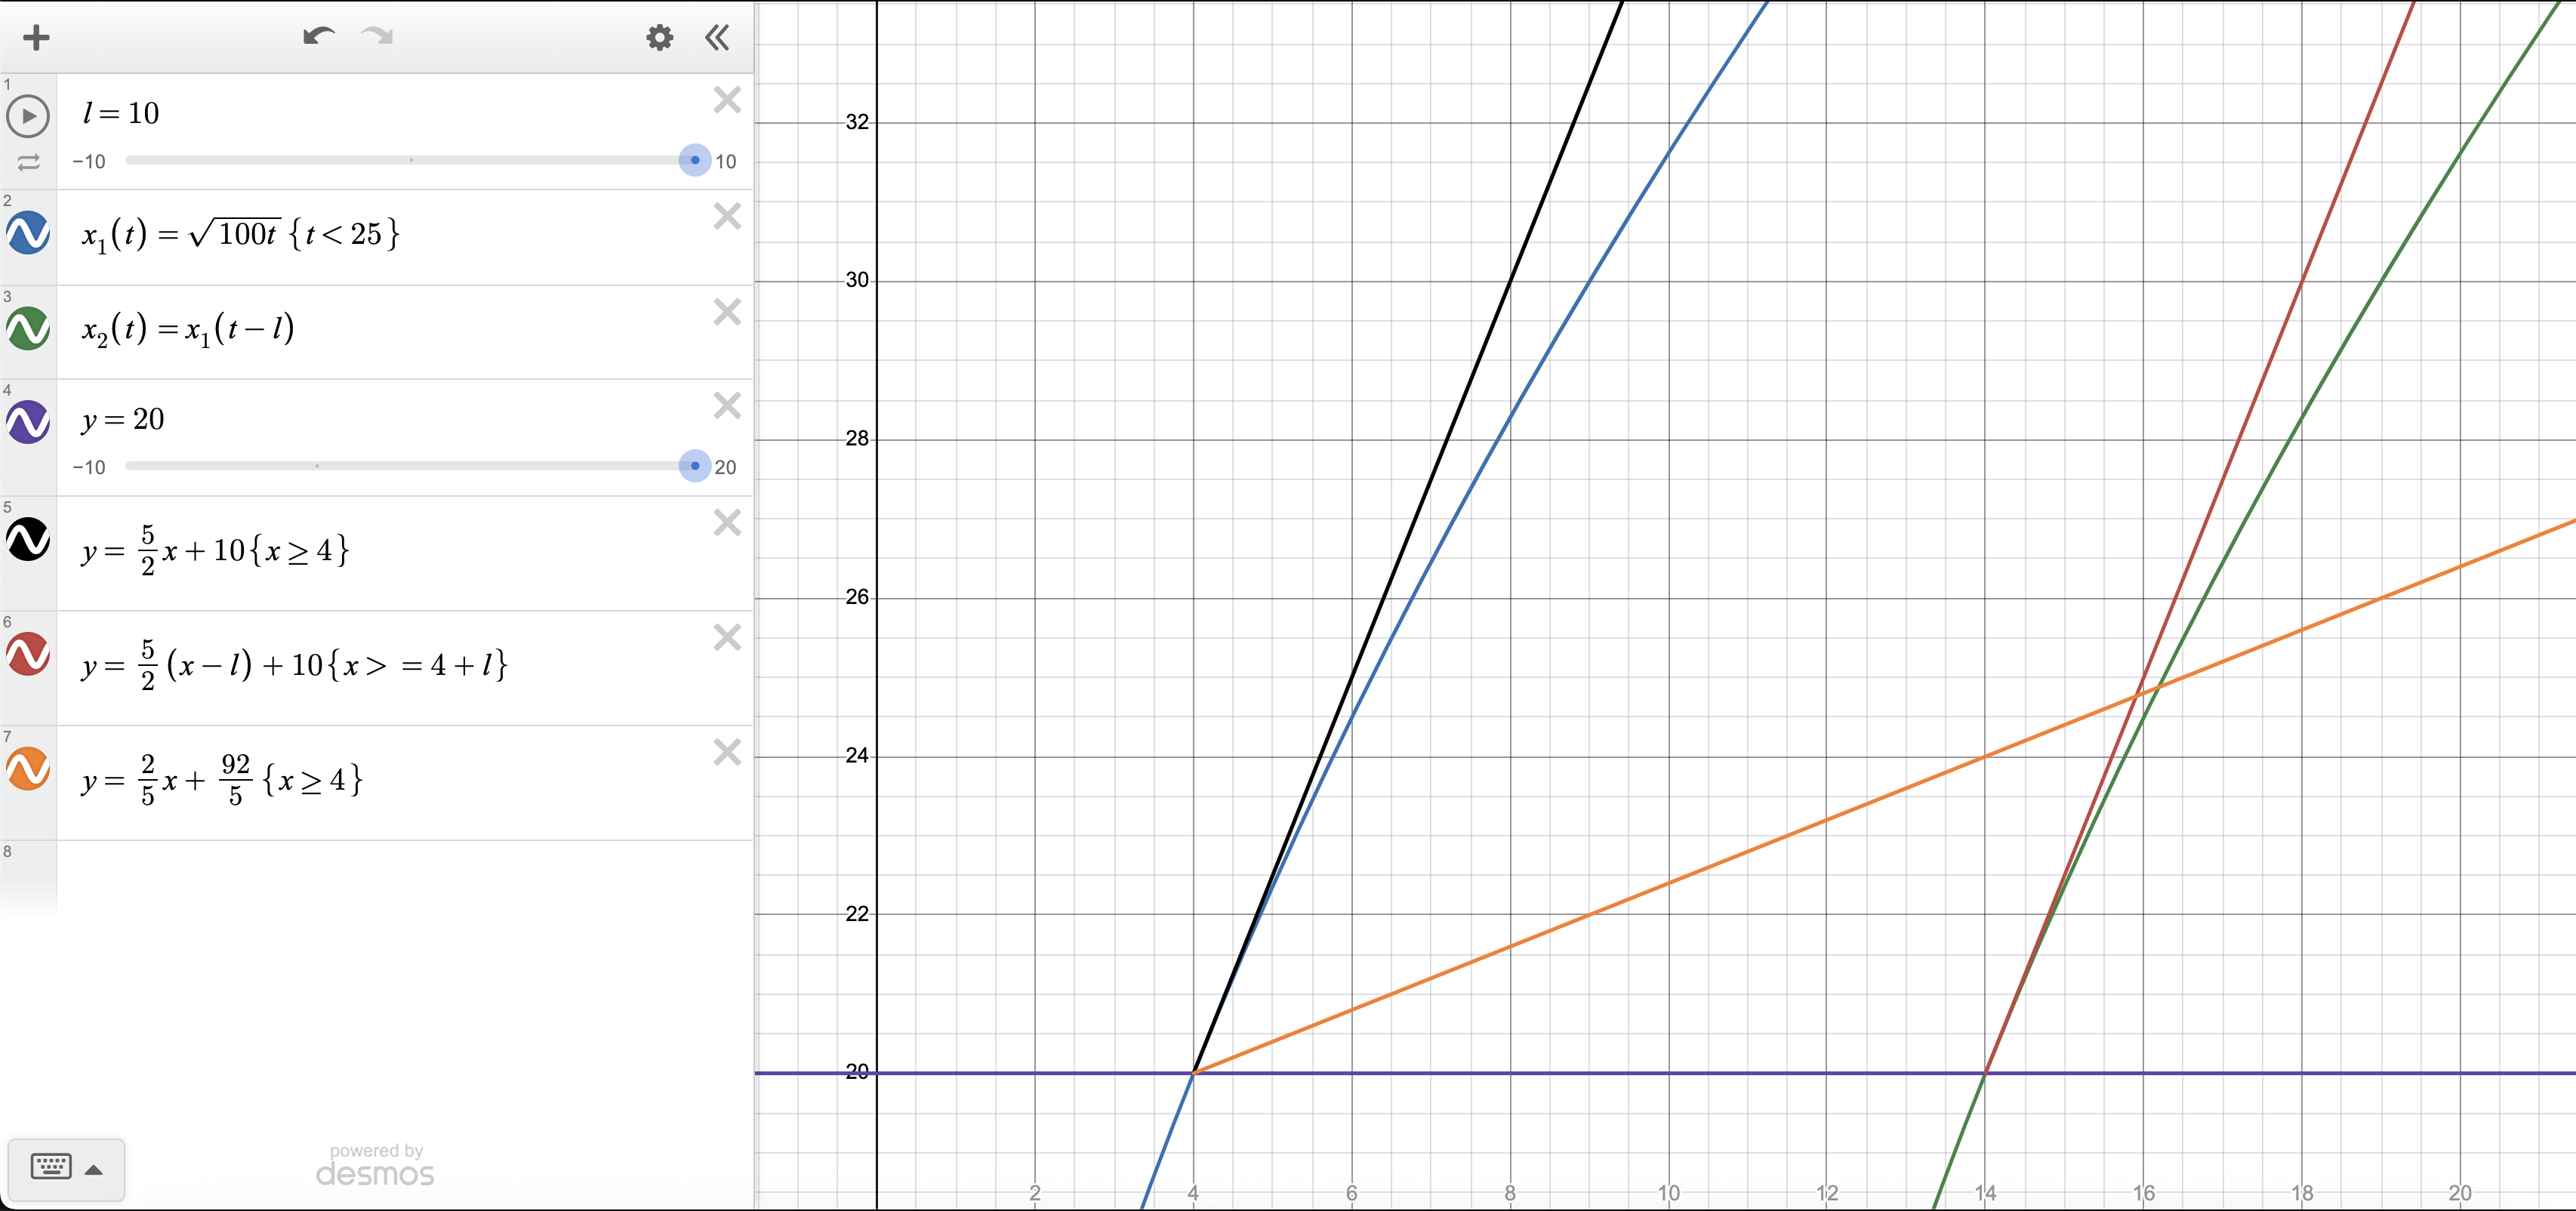
\includegraphics[width=110mm]{time2.png}
        \caption{The Spacetime Diagram of the New and Old scenarios}
    \end{center}
\end{figure}

The Blue and Green lines are the original worldlines (with acceleration), Black and Red lines are the new worldlines (without acceleration), and the Orange is the line of simultaneous events in the frame of spaceship 1 at the given moment of time $t$ (in original frame $F$).

Qualitatively, we can see that on the $x'$ axis (where at the same instant in spaceship 1's frame, or the Orange line), the position of spaceship 2 is farther when it's in the accelerated scenario, when compared to the new scenario that it stops accelerating (i.e. Green line intersects the Orange line at a farther point than the Red line did). Hence, knowing the distance (between two spaceships) in the scenario where they stopped accelerating would provide a lower bound to the distance of the actual scenario.

If we want the measurement (in spaceship 1's frame) to be at the same instant, then $\Delta t' = 0$ from the equation before. Hence, we get $0=c\Delta t' = \gamma c\Delta t-\gamma\beta\Delta x$, or $c\Delta t = \beta \Delta x$. Then, based on the coordinates showed above, in frame $F$ spaceship 2 travels an extra distance of $v\Delta t$, hence $\Delta x = \ell + v\Delta t$ (since we're measuring the x coordinate of spaceship 2 that travels with extra time $\Delta t$).

So, we get that $c \Delta t = \beta \Delta x = \beta(\ell + v\Delta t)$, hence $\Delta t = \beta\frac{\ell}{c} + \beta\cdot\frac{v}{c}\Delta t = \beta\frac{\ell}{c}+\beta^2\Delta t$. Which, $\frac{1}{\gamma^2}\Delta t = (1-\beta^2)\Delta t = \frac{\beta\ell}{c}$, or $\Delta t = \frac{\beta\ell\gamma^2}{c}$. This implies $\Delta x = \frac{c}{\beta}\Delta t = \frac{c}{\beta}\frac{\beta \ell\gamma^2}{c} = \ell\gamma^2$.

Finally, plug into the formula, we get the following: 
\begin{align}
    \Delta x' = -\gamma\beta c\Delta t + \gamma\Delta x  = -\beta^2\gamma^3\ell + \gamma^3\ell = \gamma^3(1-\beta^2)\ell = \gamma^3\cdot\frac{1}{\gamma^2}\ell = \gamma\ell
\end{align}
Hence, for the new scenario (where both ships stopped accelerating at time $t_0$ in frame $F$), at the instant in spaceship 1's frame, the two spaceships have distance $\gamma\ell$ apart, showing that the string is stretched from length $\ell$ to $\gamma\ell$. 

And, for the original scenario that the acceleration is not turned off, the stretched distance would be longer than $\gamma\ell$ in spaceship 1's frame ($\gamma\ell$ is an easier lower bound that can be derived).

\begin{comment}
and, with the coordinates of spaceship 1 being $(ct_0,\frac{1}{2}at_0^2)$ in frame $F$, then we get the following line as the set of events happening "simultaneously" in spaceship 1's frame (at that instant):
\begin{align}
    c(t - t_0) = \beta\paran*{x-\frac{1}{2}at_0^2}
\end{align}
Which, suppose at some unknown time $t=t_0+\Delta t$ (in frame $F$), spaceship 2 happens to be in one of these events, then plug in time $t$ and position $\frac{1}{2}at^2+\ell$, we get:
\begin{align}
    &c\paran*{(t_0+\Delta t)-t_0} = \beta\paran*{\frac{1}{2}a(t_0+\Delta t)^2+\ell-\frac{1}{2}at_0^2} = \beta\ell + \frac{1}{2}a\beta\Delta t(2t_0+\Delta t)\\
    &\implies c\Delta t= \beta \ell + (at_0)\beta\Delta t  + \frac{1}{2}a\beta (\Delta t)^2 = \beta \ell + \frac{\beta^2}{c}\Delta t  + \frac{1}{2}a\beta (\Delta t)^2\\
    &\implies \frac{a\beta}{2}(\Delta t)^2 + \paran*{\frac{\beta^2}{c}-c}\Delta t+\beta\ell = 0\implies (\Delta t)^2 + \frac{2(\beta^2-c^2)}{a\beta c}\Delta t+\frac{2\ell}{a}=0\\
    &\implies \Delta t = \frac{(c^2-\beta^2)}{a\beta c}\pm \sqrt{\paran*{\frac{(c^2-\beta^2)}{a\beta c}}^2-\frac{2\ell}{a}} = \frac{(c^2-\beta^2)}{a\beta c}\paran*{1\pm \sqrt{1-\frac{2\ell a\beta^2 c^2}{(c^2-\beta^2)^2}}}
\end{align}
Using spacetime diagram below, we'll choose the event that happens earlier, or the one with negative sign (since there can't have two spaceship 2 at the same instant in spaceship 1's frame). Which, we can further simplify it:
\begin{align}
    \Delta t = \frac{(c^2-\beta^2)}{a\beta c}\cdot \frac{2\ell a\beta^2c^2}{(c^2-\beta^2)^2}\cdot\frac{1}{1+\sqrt{1-\frac{2\ell a\beta^2 c^2}{(c^2-\beta^2)^2}}} = \frac{2\ell \beta c}{(c^2-\beta^2)\paran*{1+\sqrt{1-\frac{2\ell a\beta^2 c^2}{(c^2-\beta^2)^2}}}} \leq \frac{2\ell \beta c}{(c^2-\beta^2)}
\end{align}
With $\beta\in (0,1)$, this function is constantly increasing, so $\frac{2\ell \beta c}{(c^2-\beta^2)}\leq \frac{2\ell c}{c^2-1}$. Hence, the term $\Delta s$ satisfies:
\begin{align}
    (\Delta s)^2 = -c^2(\Delta t)^2 + (\Delta x)^2 = \paran*{\frac{c^2}{\beta^2}-c^2}(\Delta t)^2 = c^2\frac{1-\beta^2}{\beta^2}\frac{4\ell^2\beta^2c^2}{(c^2-\beta^2)\paran*{1+\sqrt{1-\frac{2\ell a\beta^2 c^2}{(c^2-\beta^2)^2}}}^2}
\end{align}
\begin{align}
    \implies (\Delta s)^2 \leq \frac{4\ell^2c^4}{c^2-\beta^2} \leq
\end{align}
\end{comment}

\break

\section*{6}
\begin{question}\label{q6}

    \hfil

    \begin{itemize}
        \item[(a)] Prove that the time order of two events (i.e. which one occurs at an earlier time) is the same in all inertial frames iff they can be connected by a signal traveling at or below speed $c$.
        \item[(b)] Suppose that in an inertial fram $F$ a particular signal from $A$ to $B$ can travel at velocity $v=2c$. Show that there exists an inertial fram $F'$ (whose speed relative to $F$ is less than the speed of light) in which the signal arrives at $B$ before it is sent from $A$.
    \end{itemize}
\end{question}

\textbf{Pf:}

\subsection*{(a)}
\begin{itemize}
    \item[$\implies$:] First, suppose the time order of two events $\bA, \bB$ is the same in all inertial frames (WLOG, can assume that in all inertial frame, $\bA$ happens before or simultaneous with $\bB$). Here, we set $\Delta t:=t_B-t_A \geq 0$, and same convention applies in other inertial frames also.
    
    Now, fix an inertial frame $F$ (using unprimed coordinates) with coordinates such that $\bA,\bB$ only differ in $x$-component (which the two events have $\Delta y=\Delta z=0$ in frame $F$, $\bA$ has $x$-coordinate $x$, and $\bB$ has $x$-coordinate $x+\Delta x$ for some $x,\Delta x\in\RR$). 

    Consider a Lorentz Boost in the $x$ direction with arbitrary speed $0< v<c$, then in the new inertial frame $F'$ (using primed coordinates), we get the following relation with time difference $\Delta t'$:
    \begin{align}
         \gamma c\Delta t-\gamma\beta \Delta x =c\Delta t'\geq 0\implies c\Delta t \geq \beta \Delta x
    \end{align}
    (Note: $\Delta t' = t_B' - t_A' \geq 0$ based on our assumed time order of $\bA,\bB$).

    Similarly, consider a Lorentz Boost in the $-x$ direction with the same speed $v$ from the original frame $F$, then in the new inertial frame $F''$ (using double primed coordinates), we get the following relation with time difference $\Delta t''$:
    \begin{align}
        \gamma c\Delta t + \gamma\beta \Delta x = c\Delta t'' \geq 0\implies c\Delta t \geq -\beta \Delta x
    \end{align}
    With $|\Delta x| = \Delta x$ or $|\Delta x| = -\Delta x$ (at least one equation is true), (27) and (28) shows $c\Delta t\geq \beta |\Delta x|$.

    Here, there are two situations:
    \begin{itemize}
        \item If $\Delta t=0$, then with $v>0$, $\beta =\frac{v}{c}>0$, hence $0=c\Delta t \geq \beta |\Delta x|\geq 0$ enforces $\beta |\Delta x|=0$, or $|\Delta x|=0$. Therefore, $\Delta x = 0$.
        
        Since we assume $\bA,\bB$ has spatial coordinates in $F$ differ by only $x$ component, then with $\Delta x=0$ and $\Delta t=0$, this implies $\bA=\bB$ in frame $F$, which turns out to be the same event in the spacetime. Then, they can trivially be connected by a signal traveling at or below speed $c$.

        \item Else, if $\Delta t>0$, then with $\beta >0$ (proven above), the inequality becomes:
        \begin{align}
            \frac{c}{\beta}\geq \frac{|\Delta x|}{\Delta t} \geq 0
        \end{align}
        Notice that with speed $0<v<c$ being arbitrary, $0<\beta=\frac{v}{c}<1$ is arbitrary. Hence, with $\frac{|\Delta x|}{\Delta t}\leq \frac{c}{\beta}$ for all $\beta\in (0,1)$, we get that $\frac{|\Delta x|}{\Delta t}\leq \inf_{\beta\in (0,1)}(\frac{c}{\beta}) = c$ (which means $\frac{c}{\beta}$ for $\beta\in (0,1)$ has a largest lower bound of $c$).

        Then, choose a signal with speed $u = \frac{|\Delta x|}{\Delta t}$ that propogates from the spatial coordinate of $\bA$ to spatial coordinate of $\bB$ (either in $x$ or $-x$ direction, depending on the sign of $\Delta x$), if the signal starts propogating at time $t$ (when event $\bA$ happens in frame $F$), then in frame $F$ after time $\Delta t$, the signal travels through distane $u\Delta t=|\Delta x|$, which reaches the spatial coordinates of $\bB$, and at the time $t+\Delta t$ when event $\bB$ happens in frame $F$. So, this signal can propogate from $A$ to $B$, while its speed $0\leq u = \frac{|\Delta x|}{\Delta t}\leq c$.
    \end{itemize}
    In conclusion, the above two cases show that "time order of two events is the same in all inertial frames" $\implies$ "they can be connected by a signal traveling at or below speed $c$".

    \rule{15.6cm}{0.1mm}

    \item[$\impliedby$:] Now, suppose the events $\bA,\bB$ can be connected by a signal traveling at or below speed $c$. Fix an inertial frame $F$ (unprimed), and WLOG, assume $\Delta t = t_B - t_A > 0$ (i.e. $\bA$ happens before $\bB$ in this inertial frame). 
    
    (Note: can assume $\Delta t>0$, since if $\Delta t = 0$, then in frame $F$ there's time $\Delta t=0$ for the signal to propogate, which the signal reaches nowhere but the spatial position of $\bA$, then if the signal reaches $\bB$'s spatial position within no time, $\bA$ and $\bB$ must have the same spatial position, or $\bA=\bB$ since they also have the same time coordinate).

    Which, there exists a signal with some speed $0\leq u\leq c$ in frame $F$, that propagates from spatial position of $\bA$ (starting at $t_A$ in frame $F$) to the spatial position of $\bB$ (ending at $t_B$ in frame $F$).
    
    \hfil

    Now, consider an inertial frame $F'$ with arbitrary speed $0<v<c$ relative to $F$. Choose the coordinate of $F$ and $F'$, such that the $x$ direction aligns with the relative velocity of frame $F'$ from frame $F$. In this coordinates of frame $F$, $\bA=(ct_A, x,y,z)$ for some $x,y,z\in \RR$, while $\bB = (c(t_A+\Delta t),x+\Delta x,y+\Delta y,z+\Delta z)$ for some $\Delta x,\Delta y,\Delta z\in\RR$. Then, with the signal propogates from $\bA$ to $\bB$ with displacement $(\Delta x,\Delta y,\Delta z)$ and time $\Delta t>0$ in frame $F$, we get the following about the distance traveled $\Delta r$ of the signal, and what it implies:
    \begin{align}
        &\Delta r=\sqrt{(\Delta x)^2+(\Delta y)^2+(\Delta z)^2},\quad u = \frac{\Delta r}{\Delta t} \leq c\\
        &\implies 0\leq (\Delta x)^2\leq (\Delta x)^2+(\Delta y)^2 + (\Delta z)^2=(\Delta r)^2\leq c^2(\Delta t)^2\\
        &\implies |\Delta x|\leq c|\Delta t| = c\Delta t
    \end{align}
    (Note: $\Delta r$ is the distance the signal travels).

    Which, under Lorentz Trnasformation from $F$ to $F'$, we get:
    \begin{align}
        \begin{pmatrix}
            c\Delta t'\\ \Delta x'\\ \Delta y'\\ \Delta z'
        \end{pmatrix} = \begin{pmatrix}
            \gamma & -\gamma\beta & 0&0\\
            -\gamma\beta & \gamma &0&0\\
            0&0&1&0\\0&0&0&1
        \end{pmatrix}\begin{pmatrix}
            c\Delta t\\\Delta x\\\Delta y\\\Delta z
        \end{pmatrix} = \begin{pmatrix}
            \gamma c\Delta t-\gamma\beta \Delta x\\
            -\gamma\beta c\Delta t + \gamma \Delta x\\
            \Delta y\\
            \Delta z
        \end{pmatrix}
    \end{align}
    Which, with the inequality $-|\Delta x|\leq -\Delta x$, $0<\beta = \frac{v}{c}<1$, and $|\Delta x|\leq c\Delta t$, we get the following inequality:
    \begin{align}
        &c\Delta t - \beta \Delta x \geq c\Delta t - \beta |\Delta x| > c\Delta t - |\Delta x| \geq 0\\
        &\implies \Delta t' = \frac{\gamma}{c}(c\Delta t-\gamma\beta \Delta x) > 0
    \end{align}
    Hence, we also have $t'_B - t'_A = \Delta t' >0$, showing that in frame $F'$, $\bB$ still happens after $\bA$, they still have the same time order as in frame $F$. Then, with $F'$ being an inertial frame with arbitrary nontrivial relative velocity to frame $F$ (the original frame of reference), we can claim that in all valid inertial frames, the time order of $\bA,\bB$ is preserved.

    In conclusion, "Two events can be connected by a signal traveling at or below speed $c$" $\implies$ "The time order of the two events is the same in all inertial frames".
\end{itemize}

\subsection*{(b)}
Suppose in an inertial frame $F$, a signal from $\bA$ to $\bB$ can travel at velocity $v=2c$. WLOG, can set the coordinates so that the velocity is in $x$ direction for simplicity. Also, based on the problem description, can assume that $\Delta t:= t_B-t_A >0$ (i.e. in this frame, $\bA$ happens before $\bB$). 

Then, let $\bA = (ct_A, x,y,z)$ in coordinates of frame $F$, $\bB = (c(t_A+\Delta t), x+2c\Delta t, y, z)$ in coordinates of frame $F$ (since the time difference of two events is $\Delta t$, and the signal travels at speed $2c$ in $x$ direction, which only has a displacement in $x$, with distance $2c\Delta t$).

\hfil

Now, choose a Lorentz boost in $x$ direction with speed $v = \frac{4}{5}c$ (which $\beta = \frac{v}{c}=\frac{4}{5}$, $\sqrt{1-\beta^2} = \frac{3}{5}$, and $\gamma = \frac{1}{\sqrt{1-\beta^2}}=\frac{5}{3}$). Then, after this transformation, with $\Delta x = (x+2c\Delta t)-x = 2c\Delta t$, we get the following for $\Delta t'$:
\begin{align}
    &c\Delta t' = \gamma c\Delta t - \gamma\beta \Delta x  = \frac{5}{3}\paran*{c\Delta t - \frac{4}{5}\cdot 2c\Delta t} = \frac{5}{3}c\Delta t\paran*{1-\frac{8}{5}} = -c\Delta t\\
    &\implies \Delta t' = -\Delta t<0
\end{align}
Hence, in the frame $F'$, $t'_B-t'_A = \Delta t' <0$, or $t'_B < t'_A$, showing that event $\bB$ happens before event $\bA$. Hence, the signal must arrive at $\bB$ before it is sent from $\bA$, this proves the existence of such frame (where $\bB$ receives the signal before the signal has sent from $\bA$).

\break

\section*{7}
\begin{question}\label{q7}
    A wave equation for a wave traveling at the speed of light is 
    $$\frac{\partial^2\phi}{\partial x^2}+\frac{\partial^2\phi}{\partial y^2}+\frac{\partial^2\phi}{\partial z^2}-\frac{1}{c^2}\frac{\partial^2\phi}{\partial t^2}=0$$
    Where $\phi$ is a Lorentz scalar. Show that the wave equations takes the same form after applying any of the \emph{Poincare transformations}, which consist of the Lorentz transformations and translations in each of the four directions. To avoid some algebra, you may find it useful to define 
    $$\partial_\mu \equiv \frac{\partial}{\partial r^\mu}$$
    How does $\partial_\mu$ transform under a Lorentz transformation?
\end{question}

\textbf{Pf:}

Notice that if this equation is true under both Lorentz transformations and translations in spactime, then it's also true for arbitrary compositions of the two, hence the statement would be true for all Poincare transformations.

\subsection*{1) Translations:}
Suppose the coordinates is transformed as:
\begin{align}
    (ct', x', y', z') = (c(t+t_0), x+x_0, y+y_0, z+z_0)
\end{align}
for some $x_0,y_0,z_0\in\RR$, then since $\frac{\partial r^{\mu'}}{\partial r^\mu} = 1$ for all index $\mu$, we get that $\frac{\partial \phi}{\partial r^\mu} = \frac{\partial \phi}{\partial r^{\mu'}}\frac{\partial r^{\mu'}}{\partial r^\mu} = \frac{\partial \phi}{\partial r^{\mu'}}$. Hence, the wave equation is of the same form in the frame after translation. Or, the following is true:
\begin{align}
    \frac{\partial^2\phi}{\partial x^2}+\frac{\partial^2\phi}{\partial y^2}+\frac{\partial^2\phi}{\partial z^2}-\frac{1}{c^2}\frac{\partial^2\phi}{\partial t^2}=0 \implies \frac{\partial^2\phi}{\partial (x')^2}+\frac{\partial^2\phi}{\partial (y')^2}+\frac{\partial^2\phi}{\partial (z')^2}-\frac{1}{c^2}\frac{\partial^2\phi}{\partial (t')^2}=0
\end{align}

\subsection*{2) Lorentz Boosts:}
For a more simple case, we'll consider the Lorentz Boost with speed $0<v<c$ in $x$ direction. Recall that its coordinates transformation is given as:
\begin{align}
    \begin{pmatrix}
        ct'\\x'\\y'\\z'
    \end{pmatrix} = \begin{pmatrix}
        \gamma & -\gamma\beta & 0&0\\
        -\gamma\beta & \gamma &0&0\\
        0&0&1&0\\0&0&0&1
    \end{pmatrix}\begin{pmatrix}
        ct\\x\\y\\z
    \end{pmatrix} = \begin{pmatrix}
        \gamma (ct)-\gamma\beta x\\ -\gamma\beta (ct) + \gamma x\\y\\z
    \end{pmatrix}
\end{align}
Hence, define $r^t := ct$, which for any differentiable real-valued function $\phi$ with input $(t,x,y,z)$, $\frac{\partial \phi}{\partial t}=\frac{\partial\phi}{\partial r^t} \frac{\partial r^t}{\partial t} = c\frac{\partial \phi}{\partial r^t}$ (or $\frac{\partial \phi}{\partial r^t}=\frac{\partial\phi}{\partial (ct)}=\frac{1}{c}\frac{\partial\phi}{\partial t}$), the following equality true as operators:
\begin{align}
    \frac{\partial\phi}{\partial r^\mu} = \frac{\partial\phi}{\partial r^{\mu'}}\frac{\partial r^{\mu'}}{\partial r^\mu},\quad \begin{cases}
        \frac{\partial\phi}{\partial (ct)} = \gamma\frac{\partial\phi}{\partial (ct')}-\gamma\beta\frac{\partial\phi}{\partial x'}\\
        \frac{\partial \phi}{\partial x} = -\gamma\beta\frac{\partial \phi}{\partial (ct')} + \gamma\frac{\partial\phi}{\partial x'}\\
        \frac{\partial\phi}{\partial y} = \frac{\partial\phi}{\partial y'}\\
        \frac{\partial\phi}{\partial z} = \frac{\partial\phi}{\partial z'}
    \end{cases}
\end{align}
For twice-differentiable functions (like waves for instance), we get:
\begin{align}
    \begin{cases}
        \frac{1}{c^2}\frac{\partial^2\phi}{\partial t^2}=\frac{\partial^2 \phi}{\partial (ct)^2} = \gamma^2\frac{\partial^2\phi}{\partial (ct')^2} + \gamma^2\beta^2\frac{\partial^2\phi}{\partial (x')^2} - \gamma^2\beta\frac{\partial^2\phi}{\partial(ct')\partial (x')}\\
        \frac{\partial^2\phi}{\partial x^2} = \gamma^2\beta^2\frac{\partial^2\phi}{\partial (ct')^2} + \gamma^2\frac{\partial^2\phi}{\partial (x')^2}-\gamma^2\beta\frac{\partial^2\phi}{\partial (ct')\partial (x')}\\
        \frac{\partial^2\phi}{\partial y^2}=\frac{\partial^2\phi}{\partial (y')^2}\\
        \frac{\partial^2\phi}{\partial z^2}=\frac{\partial^2\phi}{\partial (z')^2}
    \end{cases}
\end{align}
If the wave equation is true in the original frame, then in the new frame, we get:
\begin{align}
    \frac{\partial^2\phi}{\partial x^2}+\frac{\partial^2\phi}{\partial y^2} + \frac{\partial^2\phi}{\partial z^2}-\frac{1}{c^2}\frac{\partial^2\phi}{\partial t^2}=0
\end{align}
\begin{align}
    \implies &\paran*{\gamma^2\beta^2\frac{\partial^2\phi}{\partial (ct')^2} + \gamma^2\frac{\partial^2\phi}{\partial (x')^2}-\gamma^2\beta\frac{\partial^2\phi}{\partial (ct')\partial (x')}} + \frac{\partial^2\phi}{\partial (y')^2} + \frac{\partial^2\phi}{\partial (z')^2} \\ 
    &- \paran*{\gamma^2\frac{\partial^2\phi}{\partial (ct')^2} + \gamma^2\beta^2\frac{\partial^2\phi}{\partial (x')^2} - \gamma^2\beta\frac{\partial^2\phi}{\partial(ct')\partial (x')}} = 0
\end{align}
\begin{align}
    &\implies \gamma^2(1-\beta^2)\frac{\partial^2\phi}{\partial (x')^2}+\frac{\partial^2\phi}{\partial (y')^2} + \frac{\partial^2\phi}{\partial (z')^2}  - \gamma^2(1-\beta^2)\frac{\partial^2\phi}{\partial (ct')^2}=0\\
    &\implies \frac{\partial^2\phi}{\partial (x')^2}+\frac{\partial^2\phi}{\partial (y')^2} + \frac{\partial^2\phi}{\partial (z')^2}  - \frac{1}{c^2}\frac{\partial^2\phi}{\partial (t')^2}=0
\end{align}
(Note: recall that $\gamma^2 = \frac{1}{1-\beta^2}$, and $\frac{\partial^2\phi}{\partial (ct')^2} = \frac{\partial}{\partial (ct')}\paran*{\frac{\partial\phi}{\partial (ct')}} = \frac{1}{c}\frac{\partial}{\partial t'}\paran*{\frac{1}{c}\frac{\partial\phi}{\partial t'}}=\frac{1}{c^2}\frac{\partial^2\phi}{\partial (t')^2}$).

Hence, the wave equation is still true under a Lorentz Boost.

\subsection*{3) Spatial Rotations:}
We want to generalize Lorentz Boost into arbitrary Lorentz Transformation (which is always a composition of spatial rotations and Lorentz Boost, if the orientation of the vectors remain the same). Hence, it suffices to check any spatial rotation matrix (i.e. only change the spatial basis, but not the time). More generally, if $U$ is an arbitrary unitary matrix of $\RR^{3\times 3}$ (which includes all rotation matrices), then the spatial unitary transformation is:
\begin{align}
    \begin{pmatrix}
        ct'\\x'\\y'\\z'
    \end{pmatrix}=\left(\begin{array}{c|c}
        1 & 0\\
        \hline
        0 & U
    \end{array}\right)\begin{pmatrix}
        ct\\x\\y\\z
    \end{pmatrix}
\end{align}
So, we get that $t' = t$, and $r^{\mu'} = u_{\mu'\mu}r^\mu$ (where $\mu'$ represents the row of $U$ corresponding to the basis $x',y',z'$, and $\mu$ represents the column corresponding to $x,y,z$ instead). Hence, for $\mu=x,y,z$, we get the following equations for wave $\phi$:
\begin{align}
    &\frac{\partial\phi}{\partial r^\mu} = \frac{\partial\phi}{\partial r^{\mu'}}\frac{\partial r^{\mu'}}{\partial r^\mu} = u_{\mu'\mu}\frac{\partial\phi}{\partial r^{\mu'}}\\
    &\implies \frac{\partial^2\phi}{\partial (r^\mu)^2} = u_{\mu'\mu}u_{\nu'\mu}\frac{\partial^2\phi}{\partial r^{\mu'}\partial r^{\nu'}}
\end{align}
Hence, we get the following when summing up the partials of $x,y,z$ (using summation notation instead of index notation for calculation simplicity):
\begin{align}
    \sum_{\mu \in \{x,y,z\}}\frac{\partial^2\phi}{\partial (r^\mu)^2} &= \sum_{\mu\in\{x,y,z\}}\sum_{\mu'\in\{x',y',z'\}}\sum_{\nu'\in\{x',y',z'\}}u_{\mu'\mu}u_{\nu'\mu}\frac{\partial^2\phi}{\partial r^{\mu'}\partial r^{\nu'}}\\
    &= \sum_{\mu\in\{x,y,z\}}\sum_{\mu'=\nu'}(u_{\mu'\mu})^2\frac{\partial^2\phi}{\partial (r^{\mu'})^2} + \sum_{\mu\in \{x,y,z\}}\sum_{\mu'\neq \nu'}u_{\mu'\mu}u_{\nu'\mu}\frac{\partial^2\phi}{\partial r^{\mu'}\partial r^{\nu'}}
\end{align}
Now, recall that $U$ is a unitary matrix, then it means the set of its row vectors forms an orthonormal basis. Hence, for the first sum above, if fixing $\mu'$ and sum over $\mu\in\{x,y,z\}$, we get $\sum_{\mu\in\{x,y,z\}}(u_{\mu'\mu})^2 = 1$ (since it is the norm square of $(u_{\mu'x},u_{\mu'y},u_{\mu'z})$, a row vector of $U$ which has norm $1$); then, for the second summation, if fixing $\mu', \nu'$ (where $\mu'\neq \nu'$), we get $\sum_{\mu\in\{x,y,z\}}u_{\mu'\mu}u_{\nu'\mu}=0$ (since this sum represents the dot product $(u_{\mu'x},u_{\mu'y},u_{\mu'z})\cdot (u_{\nu'x},u_{\nu'y},u_{\nu'z})$; with $\mu'\neq \nu'$, the two are distinct row vectors, then with orthogonality, the dot product is $0$). 

Then,the second sum above is identically $0$, while the first sum reduces to the sum over $\mu'$. So, the above becomes:
\begin{align}
    \sum_{\mu\in \{x,y,z\}}\frac{\partial^2\phi}{\partial (r^\mu)^2} = \sum_{\mu'\in\{x',y',z'\}}
\frac{\partial^2\phi}{\partial (r^{\mu'})^2}\end{align}
Which, with $t=t'$, we get the following equation:
\begin{align}
    &\paran*{\frac{\partial^2\phi}{\partial x^2}+\frac{\partial^2\phi}{\partial y^2}+\frac{\partial^2\phi}{\partial z^2}}-\frac{1}{c^2}\frac{\partial^2\phi}{\partial t^2} = 0 \implies \paran*{\frac{\partial^2\phi}{\partial(x')^2}+\frac{\partial^2\phi}{\partial (y')^2}+\frac{\partial^2\phi}{\partial (z')^2}}-\frac{1}{c^2}\frac{\partial^2\phi}{\partial (t')^2} = 0
\end{align}
Hence, the wave equation is also in the same form under any spatial unitary transformation (which in particular is true for spatial rotation).

\hfil

Since we've verified that under arbitrary translation of spacetime, Lorentz Boost, and Spatial Rotation, the wave equation all takes the same form, then under any Poincare Transformation (which is the composition of Lorentz Transformation and translation, while Lorentz Transformation is a composition of Lorentz Boost and Spatial rotation), the wave equation still maintains in the same form.

\end{document}